\subsection{Printing The Layout:}

Once we were happy with our schematic on our computer, we match the size of the diagram on the software so that both the circuit board and the paper will have the needed sizes. For our circuit the sizes are {\itshape 9mm} of width and {\itshape 5.7mm} of height. \hfill \break

We print it out on a glossy paper, such as magazine paper. We ensure the circuit is mirrored before doing this (most PCB layout programs have this as an option when printing). Once printed, we make sure to do not touching the ink part on the paper as it can get on our hands. Then, we align the circuit diagram on the paper with the circuit board (the diagram should be facing the copper part of the circuit board) as we can see in Figure 3.2.0 and Figure 3.2.1. We start up our iron and wait until it heats up. Once heated, we carefully place the iron for around 30-45 seconds on top of the paper which is on top of the circuit board ( Figure 3.2.2 and Figure 3.2.3 ). \hfill \break

\begin{figure}[H]
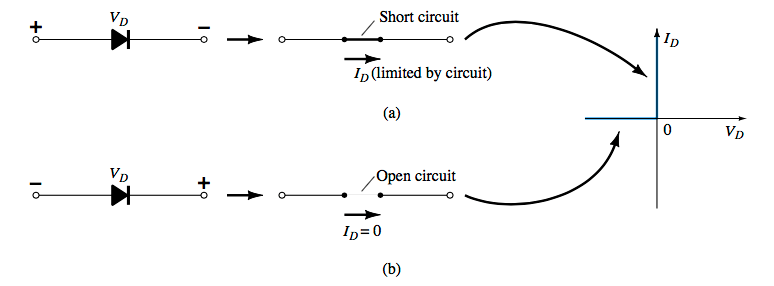
\includegraphics[height = 6cm, width = 16.5cm]{3.png}
\centering \linebreak \linebreak {\small Figure 3.2.0: Aligning the circuit diagram and the circuit board.}
\end{figure}

\begin{figure}[H]
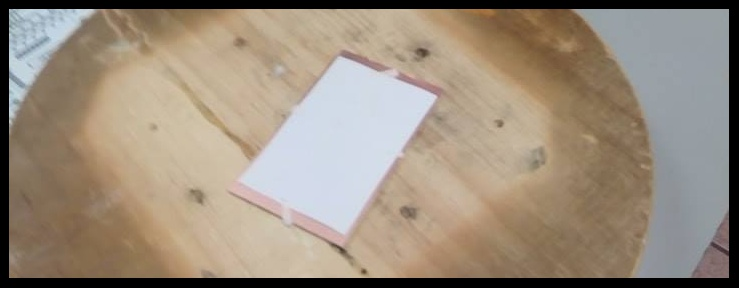
\includegraphics[height = 6cm, width = 16.5cm]{1c.jpg}
\centering \linebreak \linebreak {\small Figure 3.2.1: Aligning the circuit diagram and the circuit board ( real ).}
\end{figure}

\begin{figure}[H]
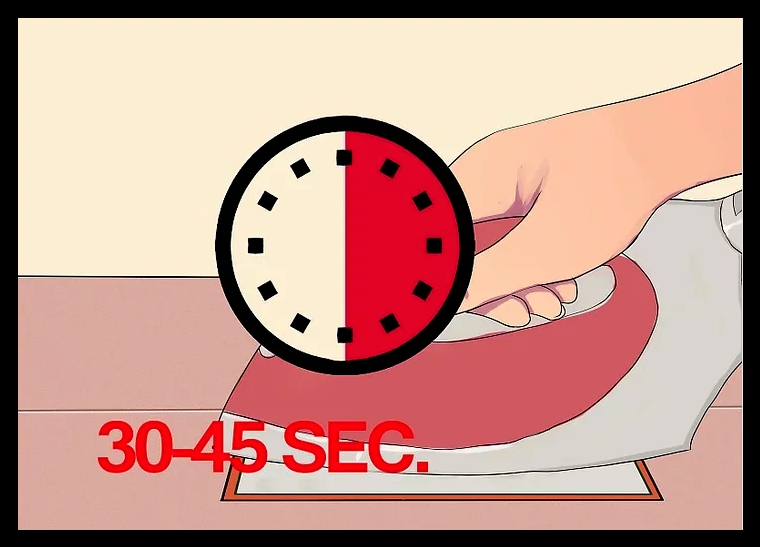
\includegraphics[height = 6cm, width = 16.5cm]{2.png}
\centering \linebreak \linebreak {\small Figure 3.2.2: Placing the iron on the circuit board.}
\end{figure} 

\begin{figure}[H]
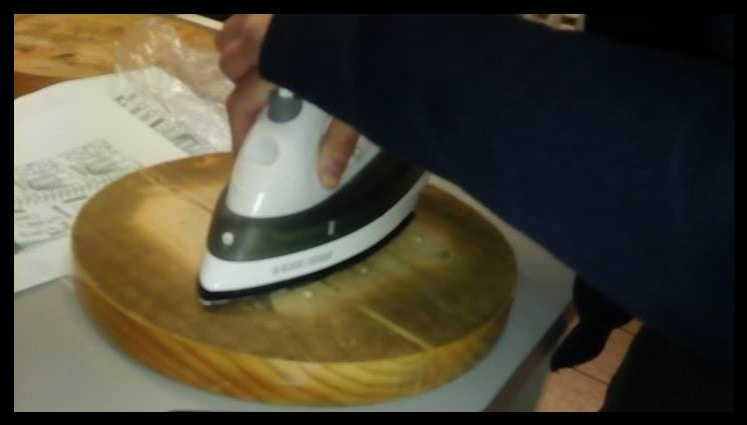
\includegraphics[height = 6cm, width = 16.5cm]{1d.jpg}
\centering \linebreak \linebreak {\small Figure 3.2.3: Placing the iron on the circuit board ( real ).}
\end{figure}

\pagebreak